\documentclass{article}
\usepackage[polish]{babel}
\usepackage[utf8]{inputenc}
\usepackage{polski}
\frenchspacing
\usepackage{indentfirst}
\usepackage{amsmath}
\usepackage{listings}
\usepackage{color}
\usepackage{hyperref}
\usepackage{graphicx}
\hypersetup{colorlinks=true}
\title{Sprawozdanie z numerycznych metod rozwiązywania cząstkowych równań rózniczkowych}
\author{Karol Urbański}
\begin{document}
\maketitle
\section{Podstawy teoretyczne}
\subsection{Rozwiązywany problem}
Rozwiązywany problem to zadanie 1 z laboratorium, w którym znajdujemy rozwiązanie \emph{równania Laplace'a} 
w przestrzeni dwuwymiarowej $(x,y)\in [0,1]^2$:
	\begin{equation}
		\frac{\delta^2 V}{\delta x^2}
			+
		\frac{\delta^2 V}{\delta y^2}
			=
		0
	\label{base}
	\end{equation}
z następującymi warunkami początkowymi:
	\begin{equation*}
		\forall x,y \in R: V(x,0)=V(x,1)=V(0,y)=V(1,y)=0,
	\end{equation*}
	\begin{equation*}
		\forall (x,y) \in C: V(x,y)=l,
	\end{equation*}
gdzie $C$ to kwadratowy obszar przewodnika taki, że $C \in [0,1]^2$,
a $l$ to dana stała oznaczająca potencjał przewodnika.
\subsection{Dyskretyzacja problemu}
Przestrzeń, w której rozwiązujemy równanie, musimy udyskretyzować, aby móc wykorzystać metody
numeryczne do przybliżenia rozwiązania problemu. Dyskretyzacji dokonujemy poprzez podział przestrzeni
na siatkę $(n-1)^2$ punktów $p_{ij} \in [0,1]^2$ takich, że $\forall (i,j) \in \{1,2,...,n-1\}\times \{1,2,...,n-1\}: p_{ij}=(ih,jh), h=\frac{1}{n}$.
\newpage
\begin{figure}[h]
\begin{center}
\setlength{\unitlength}{1cm}
\begin{picture}(4,4)
	\linethickness{0.075mm}
	\multiput(0,0)(4,0){2}%
		{\line(0,1){4}}
	\multiput(0,0)(0,4){2}%
		{\line(1,0){4}}
	\put(1,1){\circle*{0.05}}
	\put(1,2){\circle*{0.05}}
	\put(1,3){\circle*{0.05}}
	\put(2,3){\circle*{0.05}}
	\put(3,3){\circle*{0.05}}
	\put(3,2){\circle*{0.05}}
	\put(3,1){\circle*{0.05}}
	\put(2,1){\circle*{0.05}}
	\put(2,2){\circle*{0.2}}

\end{picture}
\parbox{4in}{\emph{\caption{Przykładowa dyskretyzacja dla $n=4$, punkty oznaczone kropkami, punkty należące do przewodnika w centrum (pogrubiony); obwódka oznacza otaczający ekran}}}
\end{center}
\end{figure}

Ponieważ do rozwiązania problemu będziemy
wykorzystywać MRS\footnote{MRS - metoda różnic skończonych} dla równania stacjonarnego, dla
ułatwienia obliczeń musimy zastosować dyskretyzację w taki sposób, by zmapować siatkę dwuwymiarową
do  jednowymiarowej. Wykonujemy ją w najprostszy możliwy sposób: \[p_k=p_{ij} \iff k=i\cdot (n-1)+j \]
czyli poprzez przypisanie kolejnych indeksów kolejnym elementom w kolejnych wierszach (idąc od góry 
do dołu oraz od lewej do prawej). Przypisanie to jest bardzo proste, ale niezbędne jest zadbanie o
 dokładne przygotowanie obliczeń, aby uniknąć błędów.
\subsection{Przybliżanie pochodnych drugiego stopnia}
W MRS korzystamy z zastąpienia pochodnych ilorazem różnicowym korzystającym do obliczenia przybliżonej
wartości pochodnej przy użyciu punktów siatki znajdujących się w bezpośrednim otoczeniu badanego punktu.
W przedstawionym problemie korzystamy z drugiej różnicy centralnej dla kroku h
\begin{equation}
\frac{\delta^2 f}{\delta x^2}\approx \frac{f(x+h)+f(x-h)-2f(x)}{h^2}
\end{equation}
obliczającej przybliżoną wartość drugiej pochodnej.\footnote{Obliczona wartość jest dobrym przybliżeniem wartości drugiej
pochodnej - z dokładnością do wyrazów drugiego rzędu ( $O(h^2)$ )}
\newpage
\subsubsection{Zastosowanie ilorazów różnicowych do zadanego problemu}
Dla każdego z punktów siatki zastępujemy pochodne ilorazem różnicowym. Używamy kroku $h=\frac{1}{n} $ oraz
wcześniej wprowadzonej notacji punktów $p_{ij}$.
\begin{equation}
	\frac{\delta^2 V}{\delta x^2}=\frac{V(x_{i-1j})+V(x_{i+1j})-2V(x_{ij})}{h^2}
	\label{sub1}
\end{equation}
\begin{equation}
	\frac{\delta^2 V}{\delta y^2}=\frac{V(x_{ij-1})+V(x_{ij+1})-2V(x_{ij})}{h^2}
	\label{sub2}
\end{equation}
Podstawiając (\ref{sub1}) i (\ref{sub2}) do (\ref{base}) otrzymujemy przybliżone rozwiązanie
\begin{equation}
	\frac{V(x_{i-1j}+V(x_{ij-1})-4V(x_{ij})+V(x_{ij+1})+V(x_{i+1j})}{h^2} = 0
\end{equation}
co możemy zapisać przy użyciu naszego mapowania jako
\begin{equation}
	\frac{V(x_{k-n})+V(x_{k-1})-4V(x_{k})+V(x_{k+1})+V(x_{k+n})}{h^2} = 0 
	\label{mapowanie}
\end{equation}
Jest to układ $(n-1)^2$ równań z tylomaż niewiadomymi $V(x_{k})$. Ma on postać
\begin{equation}
	AV=b
	\label{uklad}
\end{equation}
gdzie $A$ w jednowymiarowej wersji MRS byłoby dla naszego rozwiązania macierzą piecioprzekątniową
o wartościach $\frac{-4}{h^2}$ na głównej przekątnej oraz $\frac{1}{h^2}$ na przekątnej n wierszy poniżej,
1 wiersz poniżej, 1 wiersz powyżej oraz n wierszy powyżej.\footnote{Warto zauważyć, że (\ref{mapowanie})
ma postać pozwalającą na skrócenie $h^2$, co znacznie uprości warstwę implementacyjną, ale jest bez znaczenia dla
teoretycznych rozważań.}
Takie ustawienie powodowałoby jednak, że nasze rozwiązanie brałoby wtedy na brzegach obszaru pod uwagę wartości z
pól o jedno pole w lewo bądź prawo - które nie sąsiadują z danym elementem. Dlatego, w macierzy $A$, w wierszach
$k\in in, i\in {1,2,..,n-1}$ zastępujemy wartość ponad główną przekątną zerem. Podobnie, w następnym wierszu zastępujemy
wartość pod przekątną. Ponieważ warunek brzegowy (ekran) w problemie ma potencjał równy 0, wektor wyrazów wolnych ma (na razie) postać
\begin{equation*}
b=[0,0,...,0]^T
\end{equation*}
\subsubsection{Uwzględnienie przewodnika wewnątrz obszaru}
Musimy jeszcze uwzględnić źródło potencjału - przewodnik. By to zrobić, w wektorze wyrazów wolnych wiersze odpowiadające
punktom siatki należącym do przewodnika zastępujemy wartością $\frac{l}{h^2}$. Następnie, by upewnić się, że wartość
potencjału w przewodniku po obliczeniach będzie dalej równa $l$ oraz niezależna od wartości w okolicznych polach, każdy wiersz
macierzy $A$ o indeksie $i$ takim, jak punkt siatki należący do przewodnika zastępujemy wierszem, w którym $A_{ii}=1$, a
każdy pozostały element wiersza $i$ jest równy $0$. Wtedy $V(x_{i})$ będzie miał zawsze wartość $l$ po zakończeniu obliczeń,
czyli pożądaną przez nas sytuację. Dodatkowo, nie musimy uwzględniać żadnych dodatkowych warunków w wektorze wolnym - 
rozwiązanie równania zrobi to za nas.
\subsection{Rozwiązanie równania}
Tak przygotowany układ równań (\ref{uklad}) musimy rozwiązać, by otrzymać nasz rozkład potencjału. 
Do rozwiązywania nie użyjemy metody eliminacji Gaussa (ani innej metody bezpośredniej), gdyż ma ona wiele
wad. Najgorszą z nich jest ogromna złożoność dla wystarczająco dużych macierzy - biorąc pod uwagę, że siatka
50x50 ma 2500 punktów, żłożoność $O(n^3)$ jest absolutnie nie do zaakceptowania dla naszego problemu, którego
ilość zmiennych rośnie kwadratowo wraz ze zmniejszeniem kroku.
Żeby uniknąć problemu gigantycznej złożoności użyjemy algorytmu iteracyjnego: metody Gaussa-Seidla. Metoda ta
w każdej sukcesywnej iteracji ulepsza przybliżenie z poprzedniej iteracji dla układu $Ax=b$, zaczynając od 
dowolnie wybranego $x_0$. Metoda ta bazuje na dekompozycji macierzy A i działa w miejscu, co jest dodatkowym
atutem metody. Jest zbieżna dla układów, w których dominują elementy na kilku przekątnych (czyli jak w naszym problemie).
W samym algorytmie wykorzystany zostanie wzór roboczy o następującej postaci:
\begin{equation}
\label{rob}
x_i^{(t+1)} = \frac{1}{a_{ii}}[b_i - \sum_{j=1}^{i-1} a_{ij}x_j^{(t+1)} - \sum_{j=i+1}^{n} a_{ij} x_j^{(t)}]
\end{equation}
Jak widać, pierwsza z sum jest liczona na podstawie wcześniej obliczonych elementów w tej samej iteracji - metoda
działa w miejscu, czyli ma znacznie mniejszą złożoność pamięciową.

Implementacja algorytmu znajduje się w warstwie implementacyjnej (rozdział \ref{impl}).

\section{Warstwa implementacyjna}
\subsection{Kernel obliczeniowy}
\subsubsection{Wykonanie}
Kernel obliczeniowy jest to program w C, przyjmujący na wejściu następujące argumenty:
\begin{enumerate}
   \item wartość początkowa $l$
   \item ilość punktów siatki wzdłuż jednego boku
   \item współrzędna $x$ lewego górnego rogu punktów siatki należących do przewodnika
   \item współrzędna $y$ lewego górnego rogu punktów siatki należących do przewodnika
   \item współrzędna $x$ prawego dolnego rogu punktów siatki należących do przewodnika
   \item współrzędna $y$ prawego dolnego rogu punktów siatki należących do przewodnika
\end{enumerate}

\subsubsection{Rozwiązywanie układu równań}
Do rozwiązania układu równań wykorzystany jest następujący algorytm. Działa do uzyskania
odpowiednio małego błędu obliczeń.
\label{impl}
\lstset{
language=C,
basicstyle=\footnotesize\ttfamily,
numbers=left,
numberstyle=\tiny,
numbersep=5pt,
stepnumber=5,
keywordstyle=\color{blue}\bfseries,
stringstyle=\color{red},
showstringspaces=false
backgroundcolor=\color{red}
}
\begin{lstlisting}
void gauss_seidel(float** mat,float* x,float* vec,int size_sqr){
	int i,j,k=0;
	float prev;
	float sum;
	float maxerr=0.01;
	while(maxerr>0.0001){
		maxerr=0.0;
		for(i=0; i<size_sqr; i++){
			prev=x[i];
			sum=0.0;
			for(j=0;j<i;j++)
				sum+=mat[i][j]*x[j];
			for(j=i+1;j<size_sqr;j++)
				sum+=mat[i][j]*x[j];
			x[i]=(vec[i]-sum)/mat[i][i];
			if(fabs(x[i]-prev)>maxerr)
				maxerr=fabs(x[i]-prev);
		}
		k++;
	}
}
\end{lstlisting} 
\subsection{Komunikacja z interfejsem graficznym}
Interfejs graficzny otrzymuje dane poprzez strumień danych bezpośrednio z programu.
Możliwe jest również użycie prekalkulowanych wartości podanych na wejściu interfejsu.
Pierwsza linia danych podana do interfejsu to typ dawanych danych (CMODE jeżeli wywołujemy
program w C, PREMODE jeżeli wykorzystujemy stare obliczenia). Następna linia w CMODE to argumenty wywołania
programu w C, a w PREMODE gotowa do wyświetlenia tablica punktów.
\subsection{Interfejs}
Interfejs napisany jest w perlu, z użyciem OpenGL. Wyświetla płytkę z odpowiednim gradientem kolorów (niebieski
dla dodatnich potencjałów, czarny dla zerowych, zielony dla ujemnych). Może wyświetlać w trybie wireframe (klawisz w),
trybie punktowym (klawisz m), oraz z wypukłościami dla wartości różnych od zera (wyświetlanie w 3D, klawisz p).
\section{Pomiary, obserwacje}
\subsection{Testy czasu wykonania}
Do pomiaru czasu wykonania użyłem skryptu shella (zsh):
\begin{lstlisting}
for i in {1 .. 10}; do
	/usr/bin/time -f '%e' ./calc 1 n 5 5 10 10 
done
\end{lstlisting}
\begin{tabular}{|c|c|c|}
\hline
ilość punktów na brzegu & $\overline{t}$ & $\sigma$ \\
\hline
10 & 0.00s & 0.00s  \\
\hline
25 & 0.127s & 0.010s  \\
\hline
50 & 3.412s & 0.023s \\
\hline
100 & 79.662s & 0.784s \\
\hline
\end{tabular}
Złożoność obliczeniowa wydaje się znajdować na poziomie $O(n^4)$. Złożoność pamięciowa to $O(n^3)$.
\subsection{Kilka rozwiązań}
\begin{figure}[ht]
\begin{center}
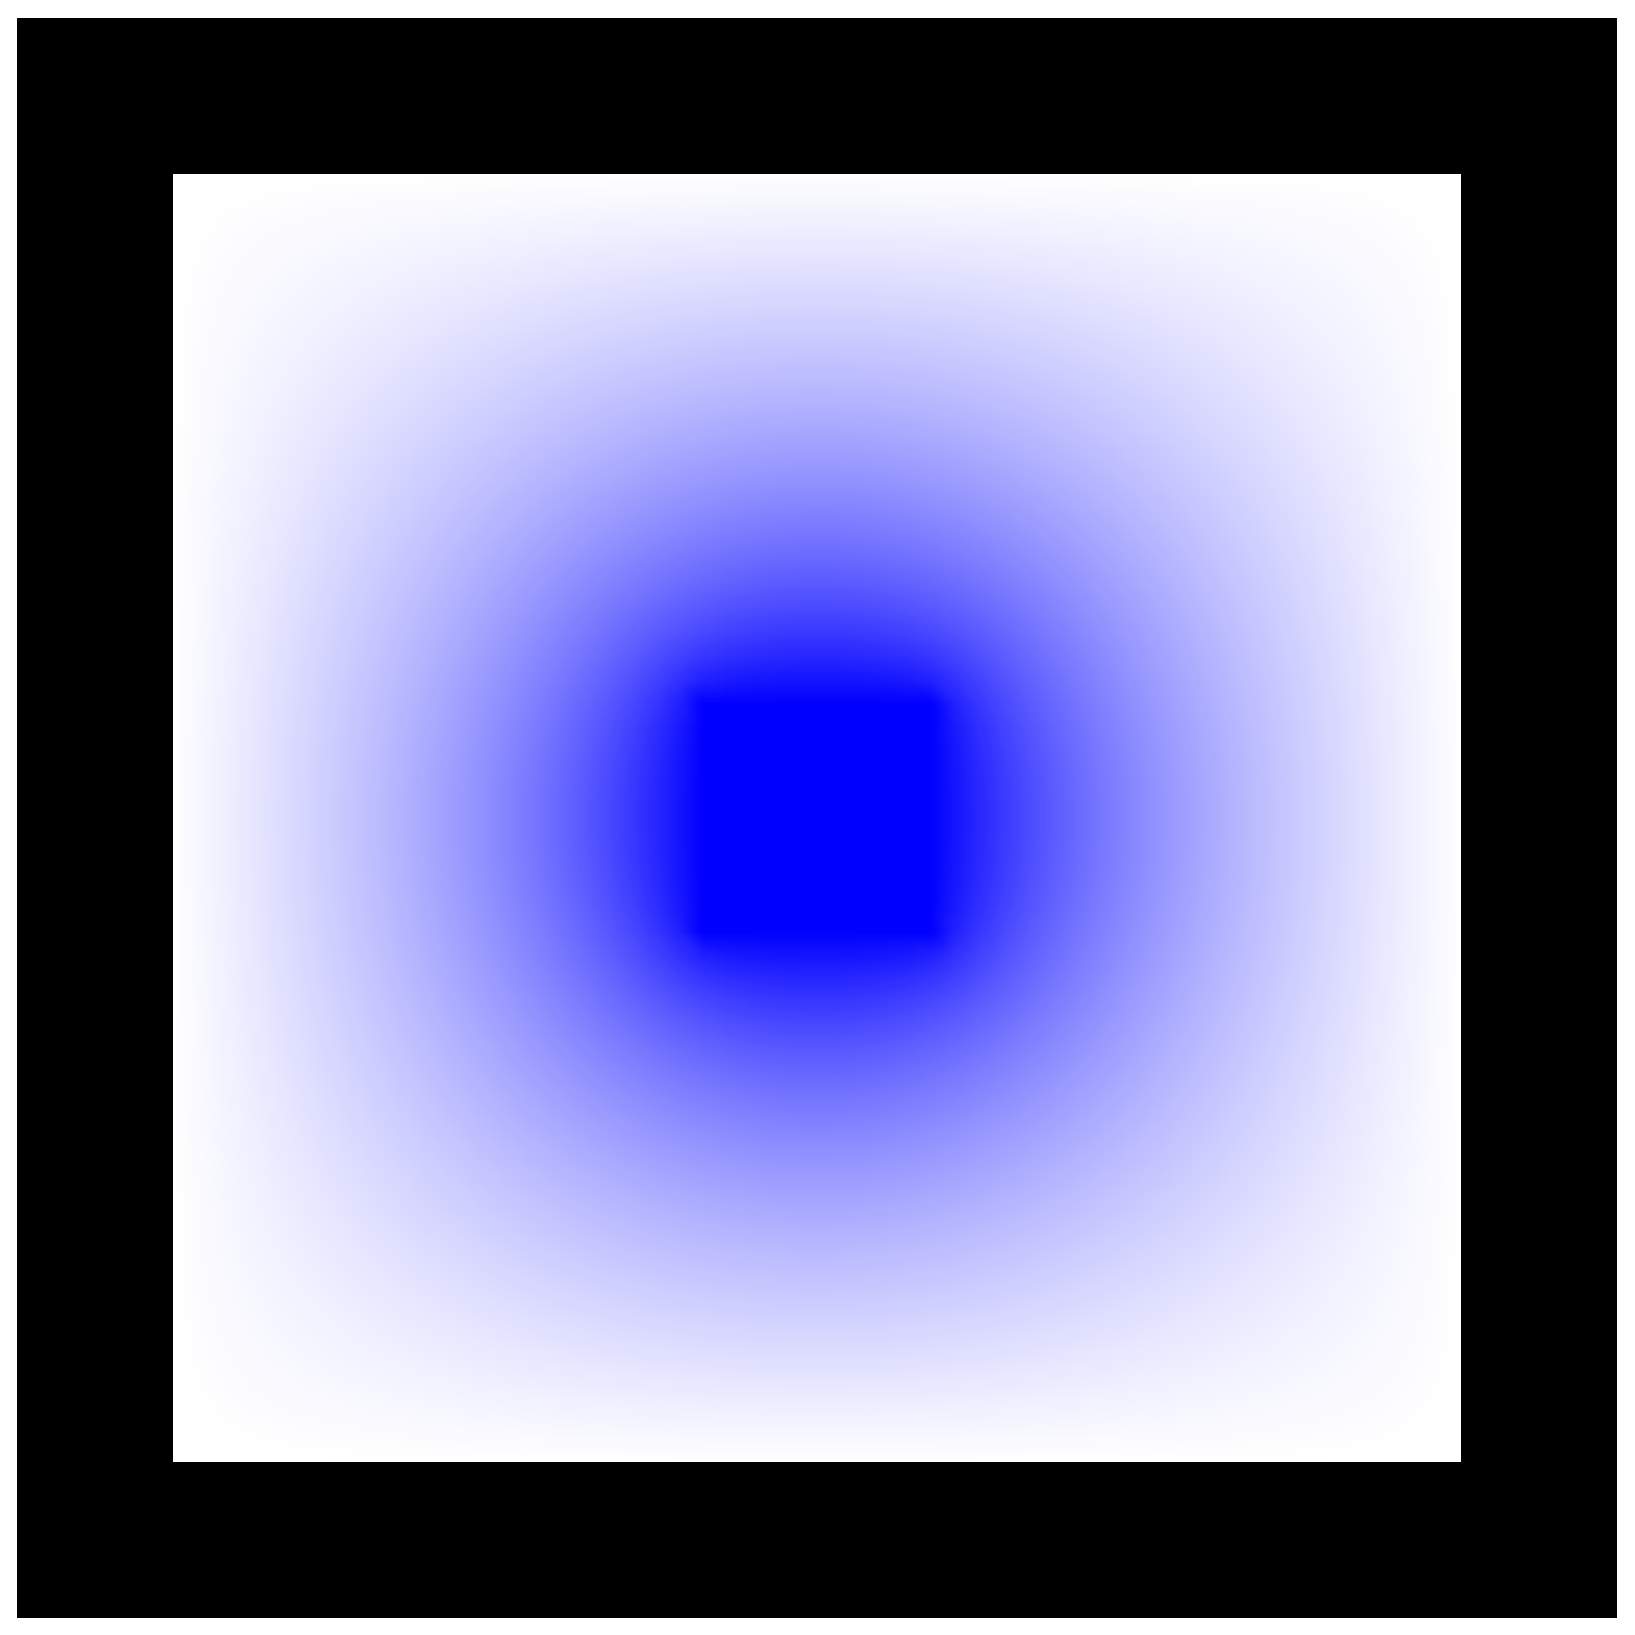
\includegraphics[scale=0.4]{im1}
\parbox{4in}{\emph{\caption{$n=50$, przewodnik o szerokości 10 punktów w środku.}}}
\end{center}
\end{figure}
\begin{figure}[ht]
\begin{center}
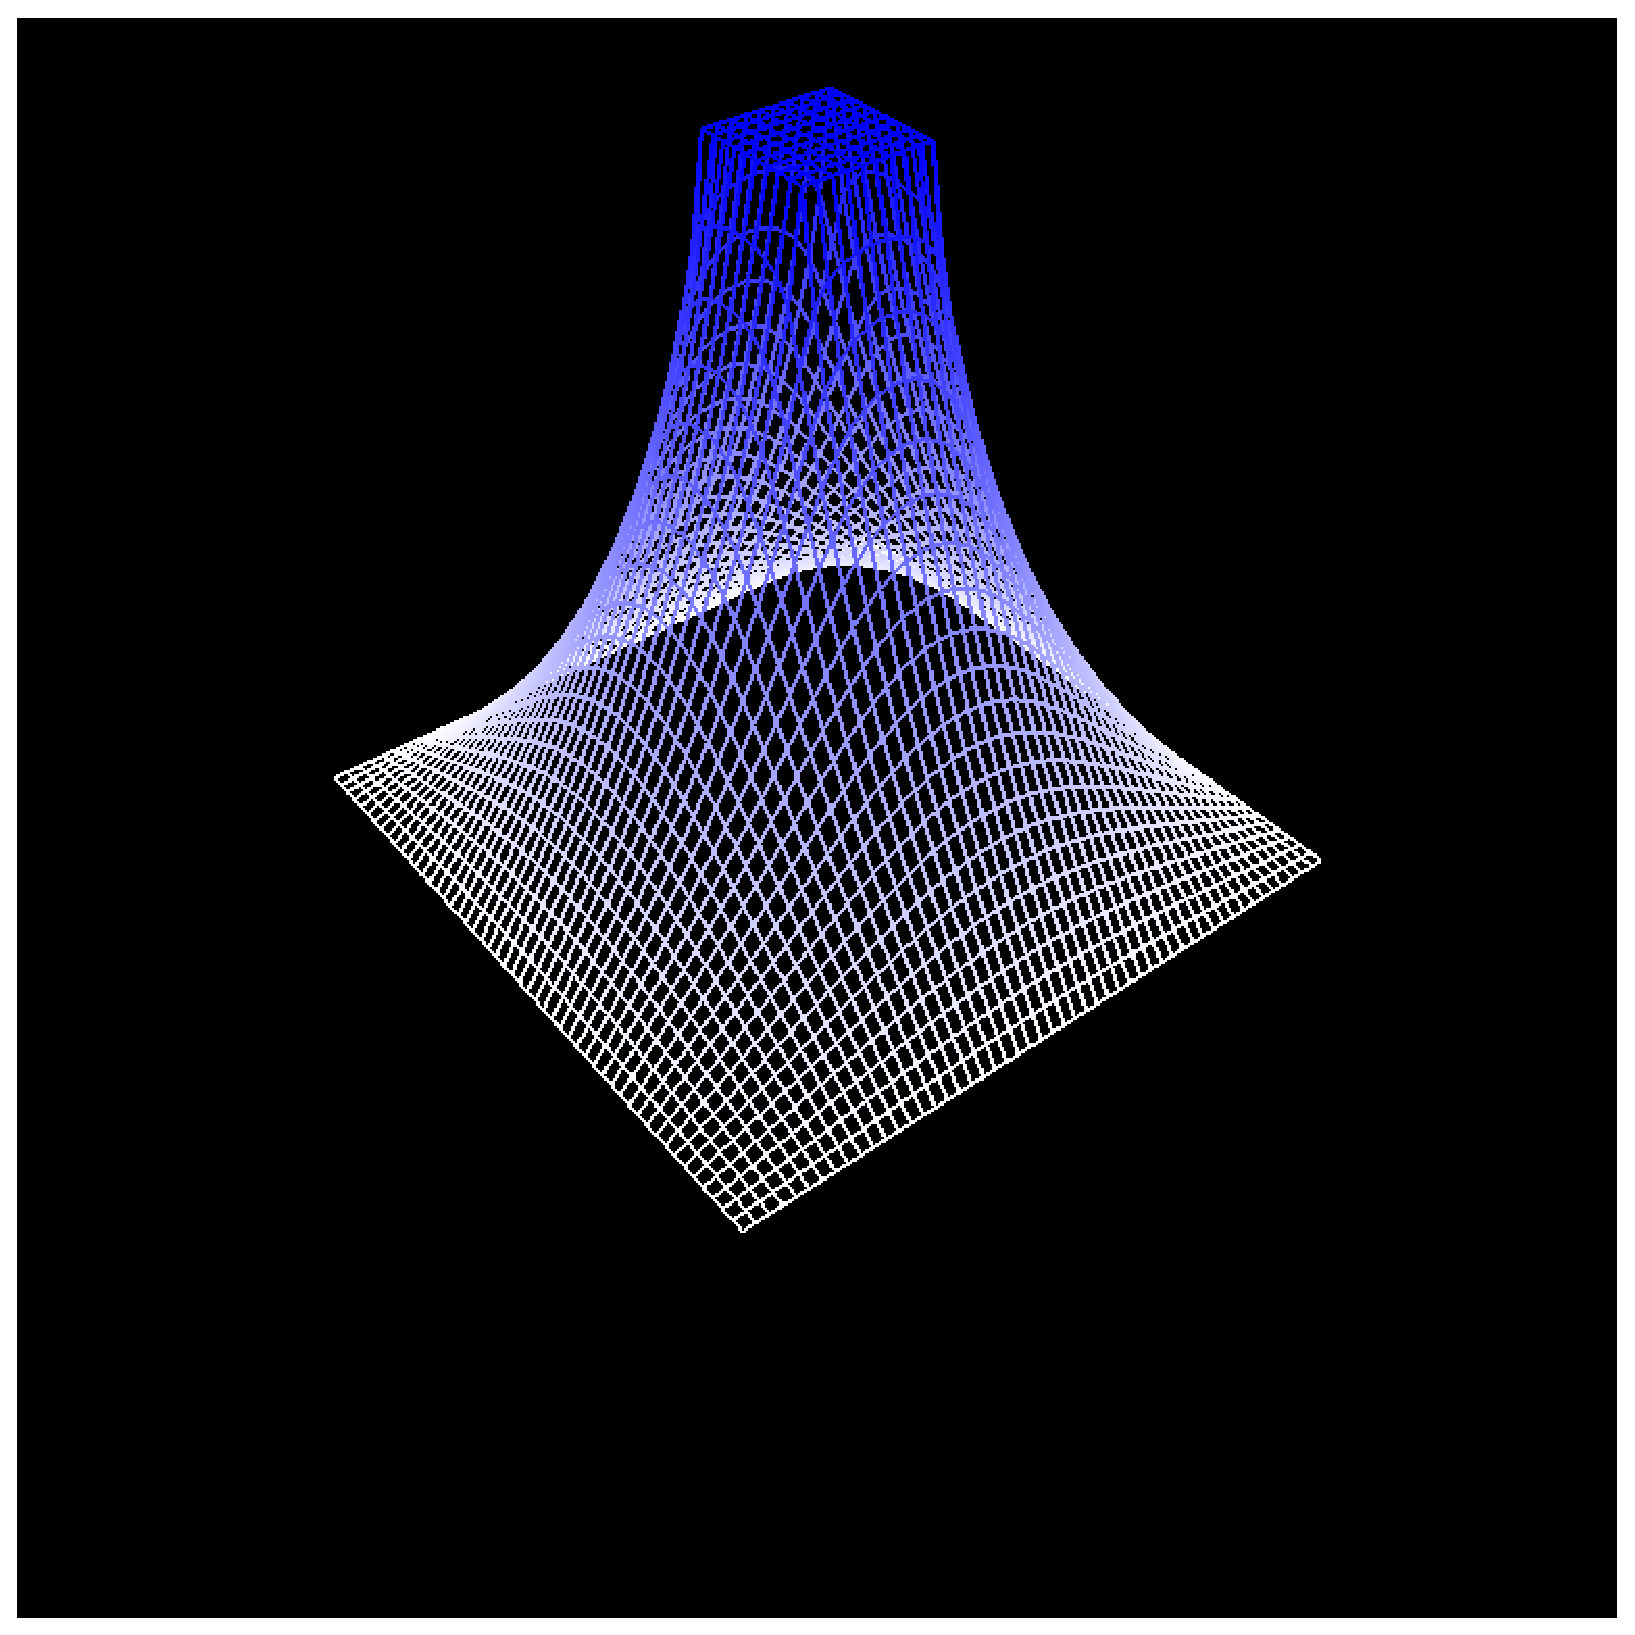
\includegraphics[scale=0.4]{im1_wire}
\parbox{4in}{\emph{\caption{$n=50$, przewodnik o szerokości 10 punktów w środku (wireframe).}}}
\end{center}
\end{figure}
\begin{figure}[ht]
\begin{center}
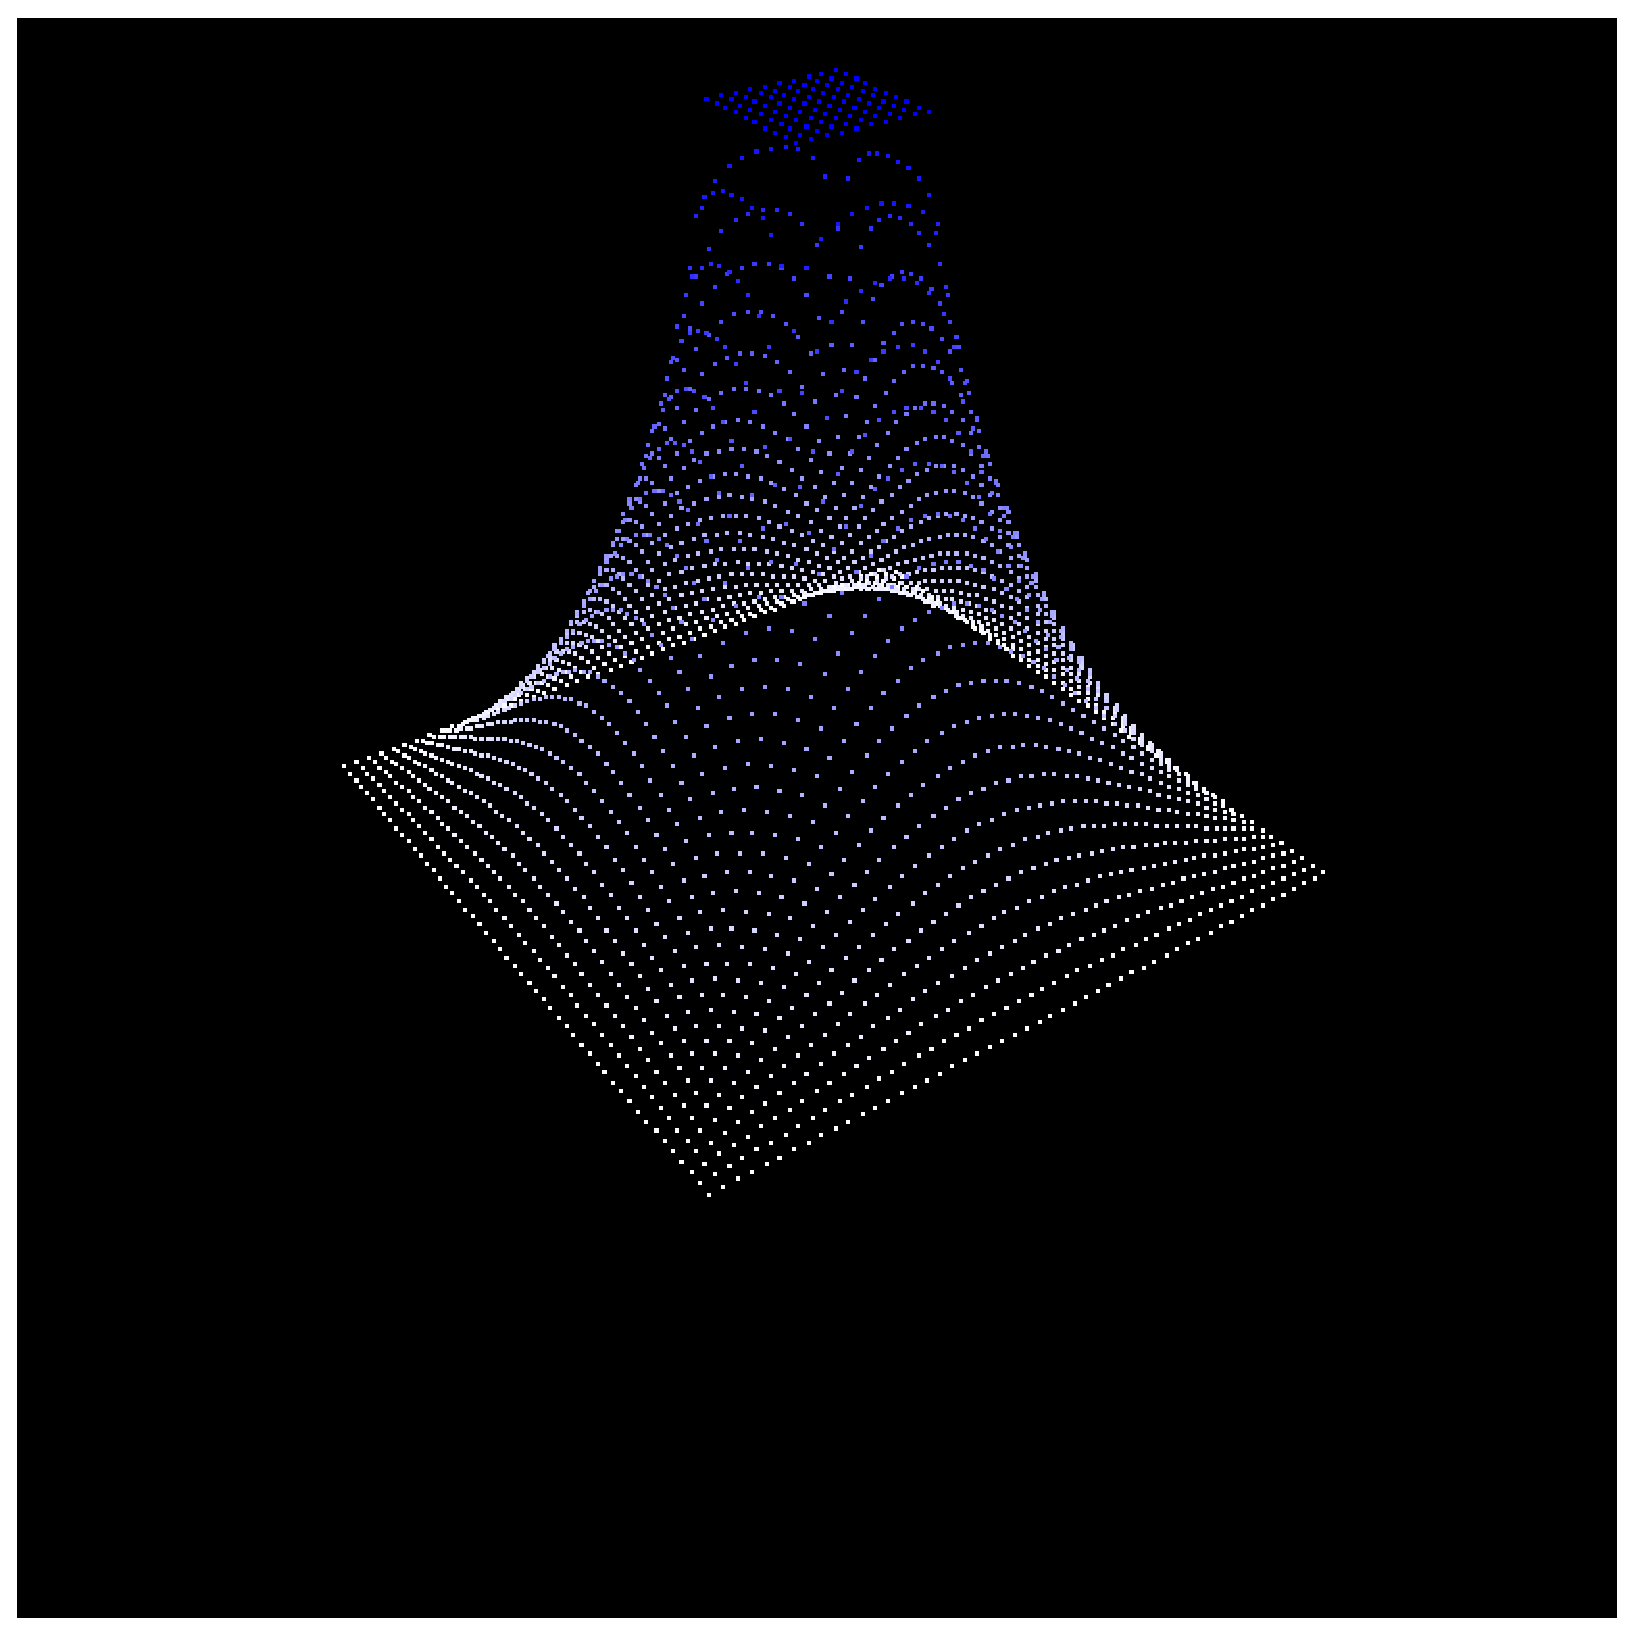
\includegraphics[scale=0.4]{im1_point}
\parbox{4in}{\emph{\caption{$n=50$, przewodnik o szerokości 10 punktów w środku (pointplot).}}}
\end{center}
\end{figure}
\begin{figure}[ht]
\begin{center}
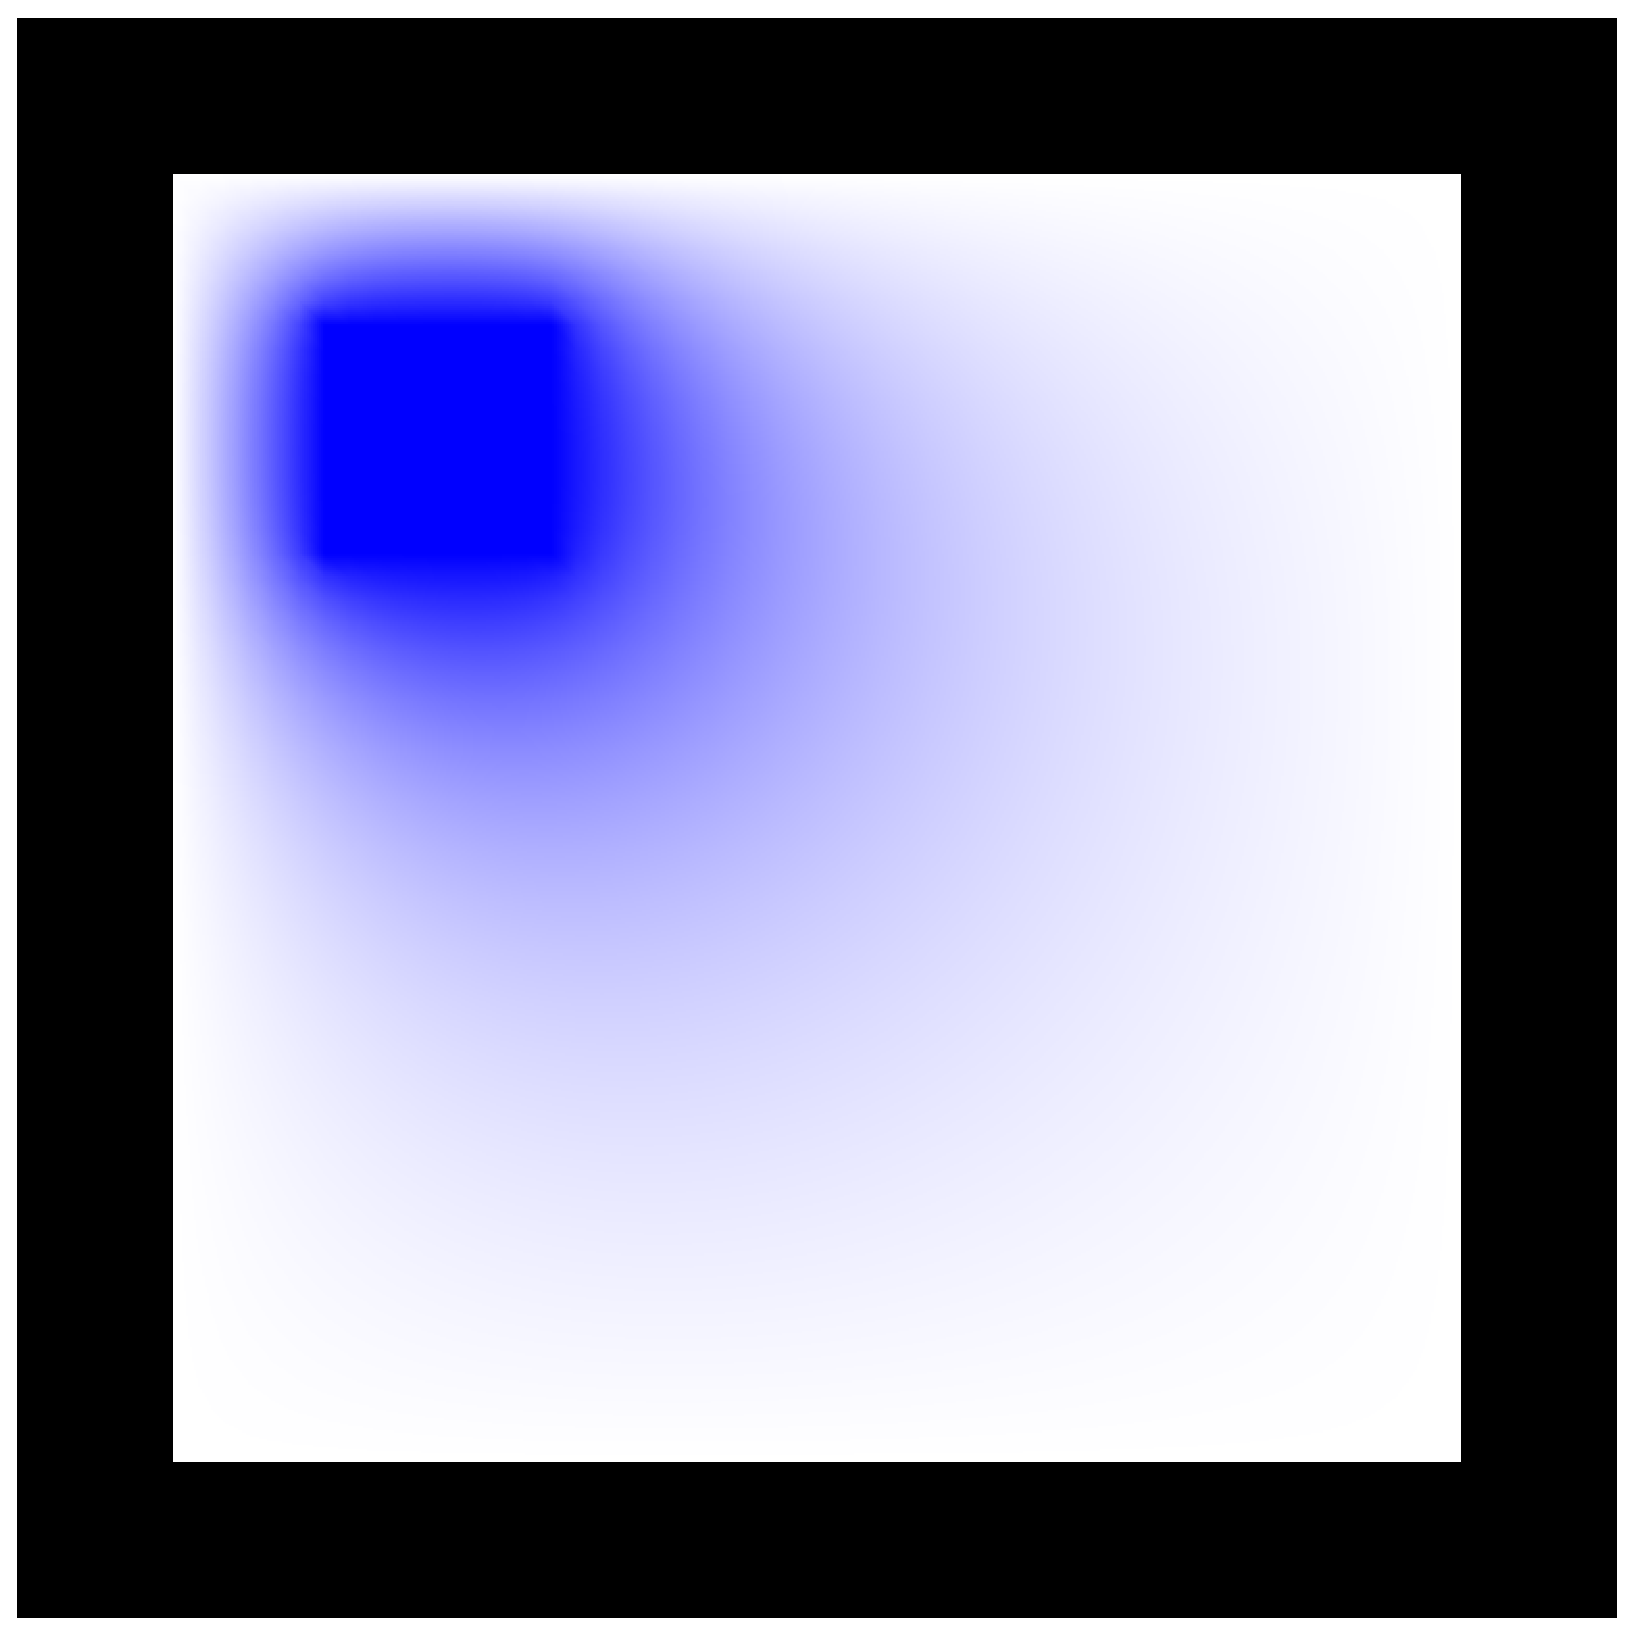
\includegraphics[scale=0.4]{im1_moved}
\parbox{4in}{\emph{\caption{$n=50$, przewodnik o szerokości 10 punktów tuż koło ekranu.}}}
\end{center}
\end{figure}
\begin{figure}[ht]
\begin{center}
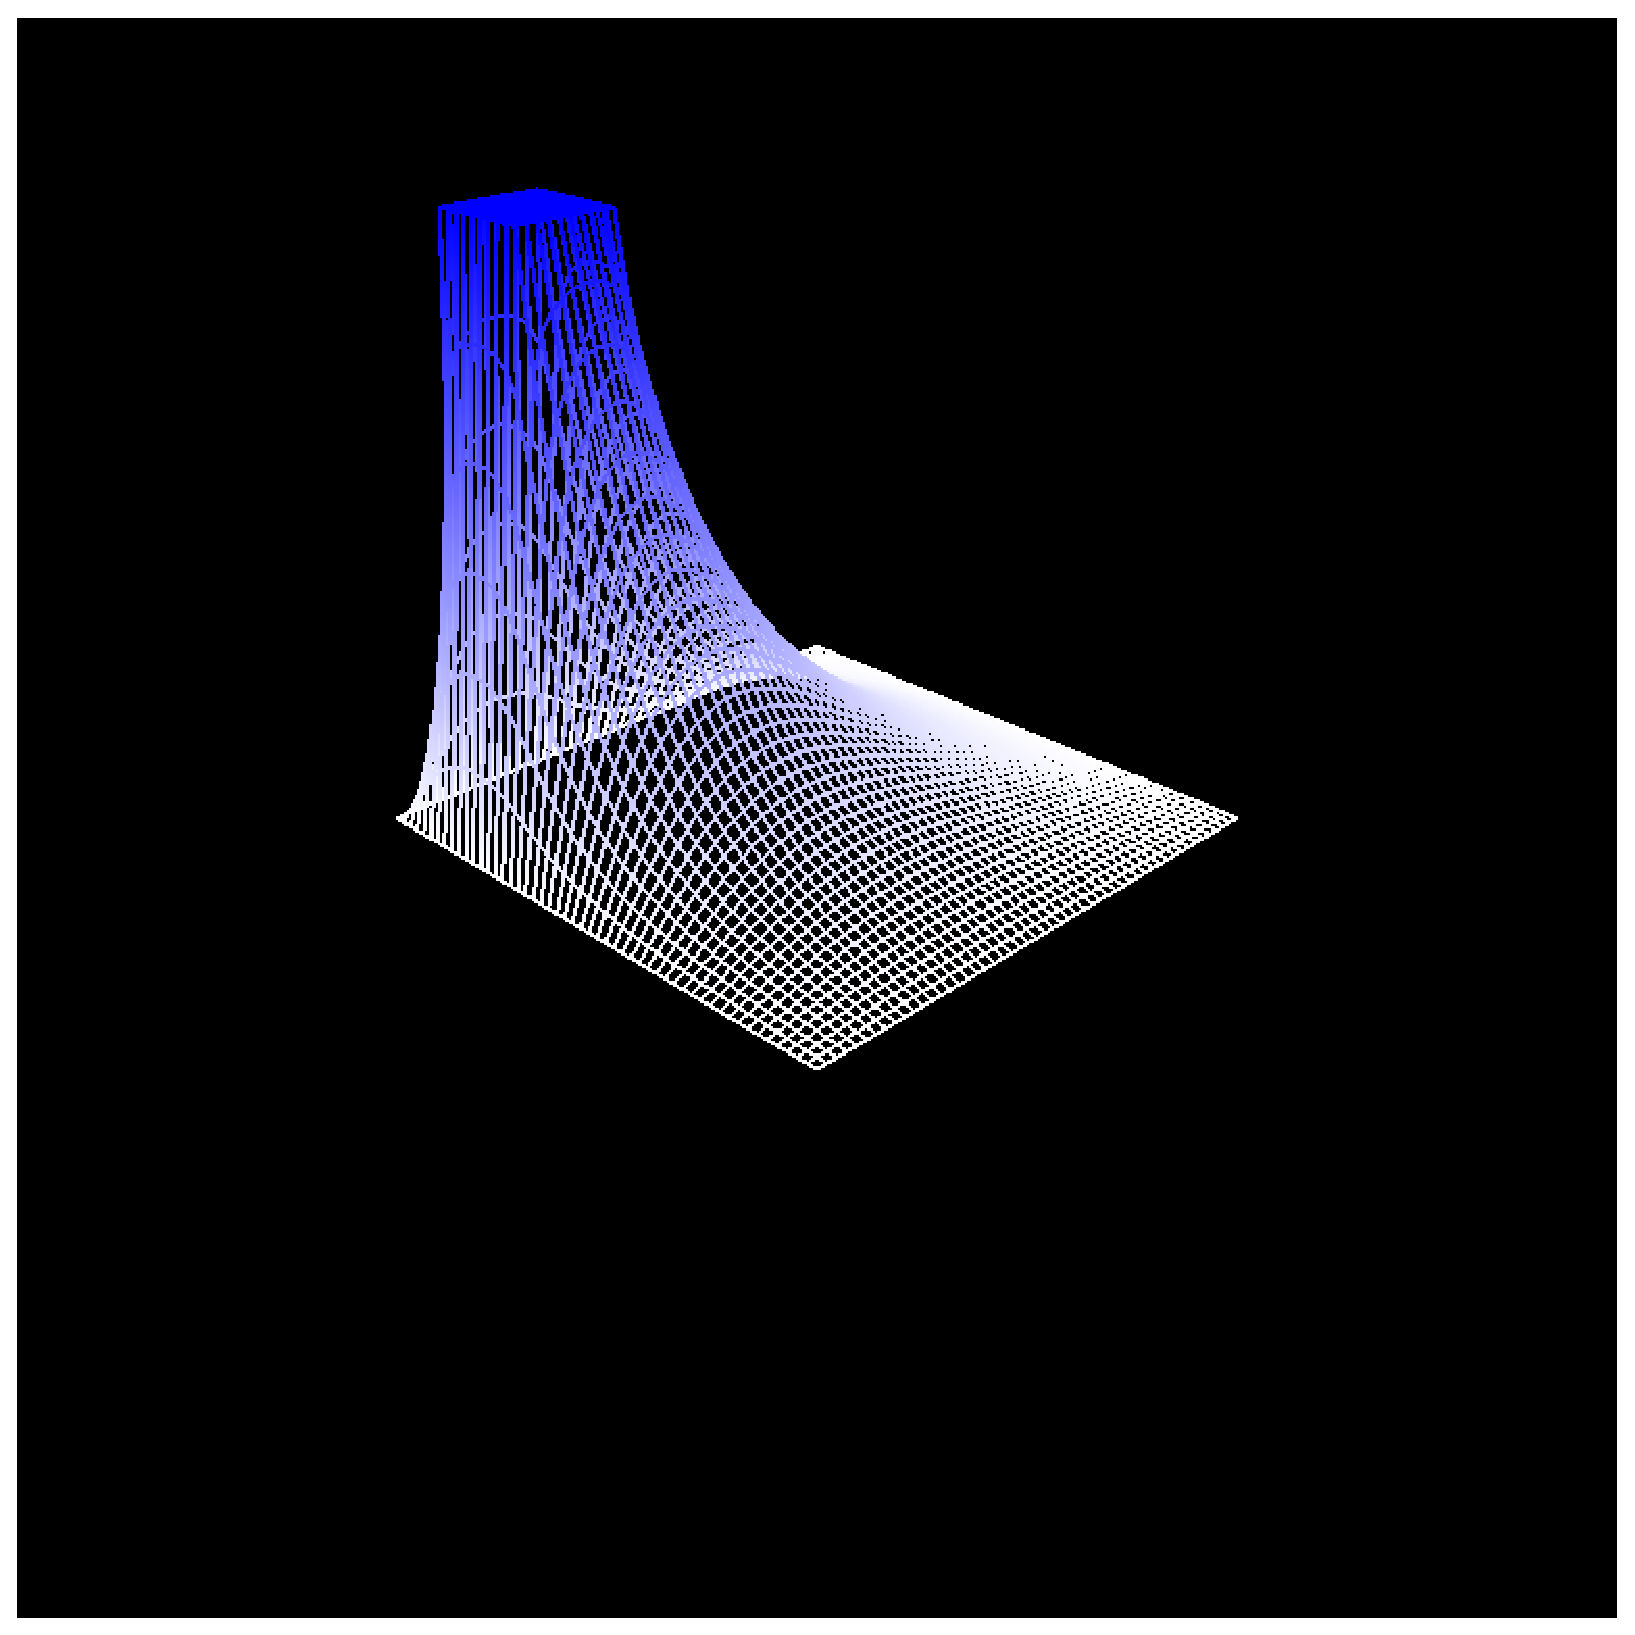
\includegraphics[scale=0.4]{im1_moved_wire}
\parbox{4in}{\emph{\caption{$n=50$, przewodnik o szerokości 10 punktów tuż koło ekranu (wireframe).}}}
\end{center}
\end{figure}
\begin{figure}[ht]
\begin{center}
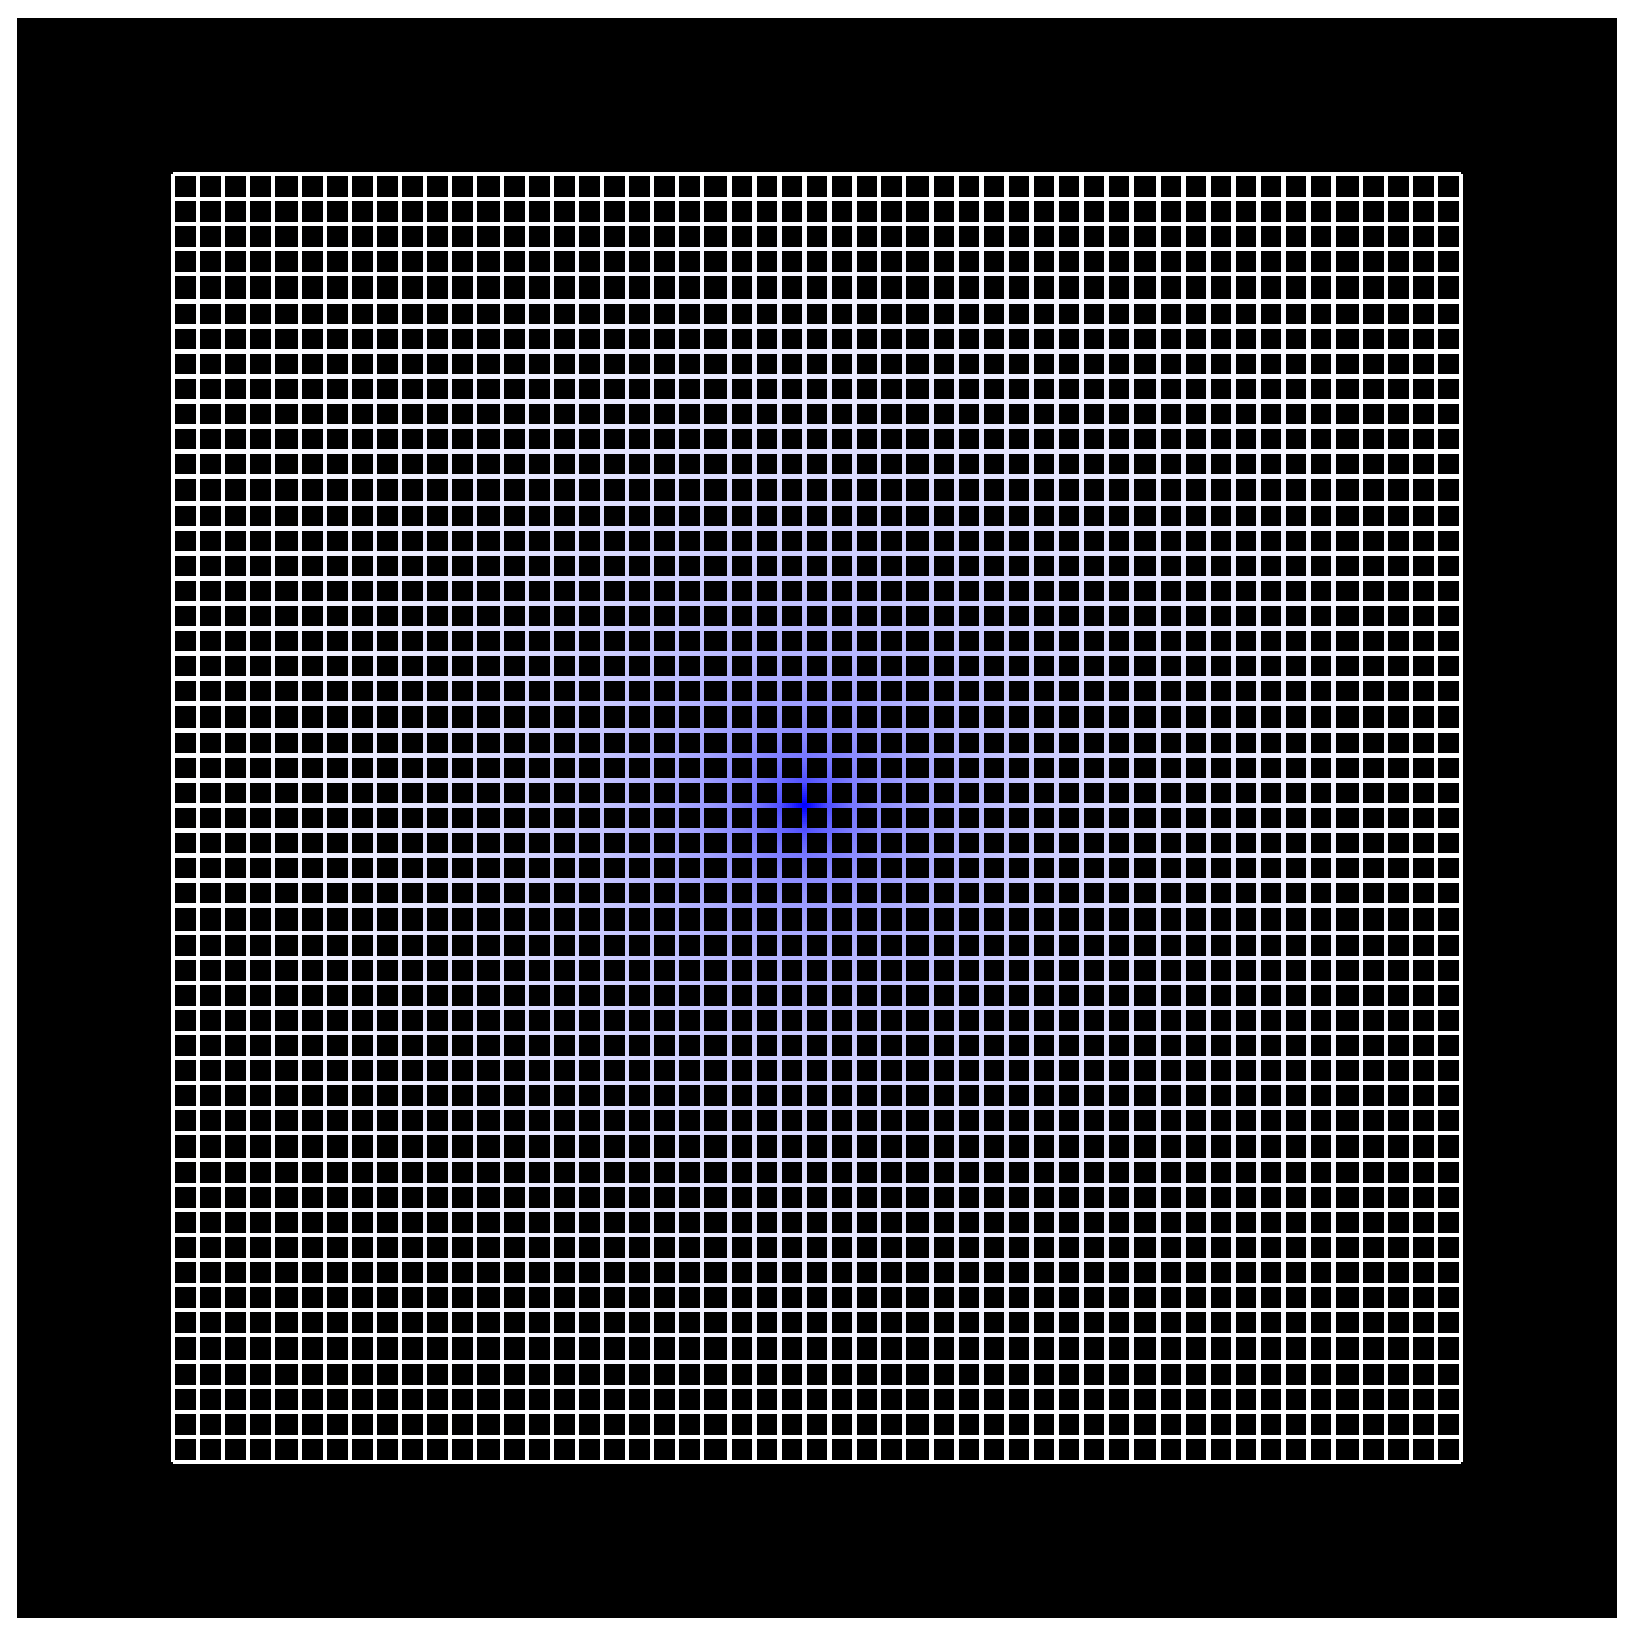
\includegraphics[scale=0.4]{im2}
\parbox{4in}{\emph{\caption{$n=50$, przewodnik o szerokości 1 punktu w środku.}}}
\end{center}
\end{figure}
\begin{figure}[ht]
\begin{center}
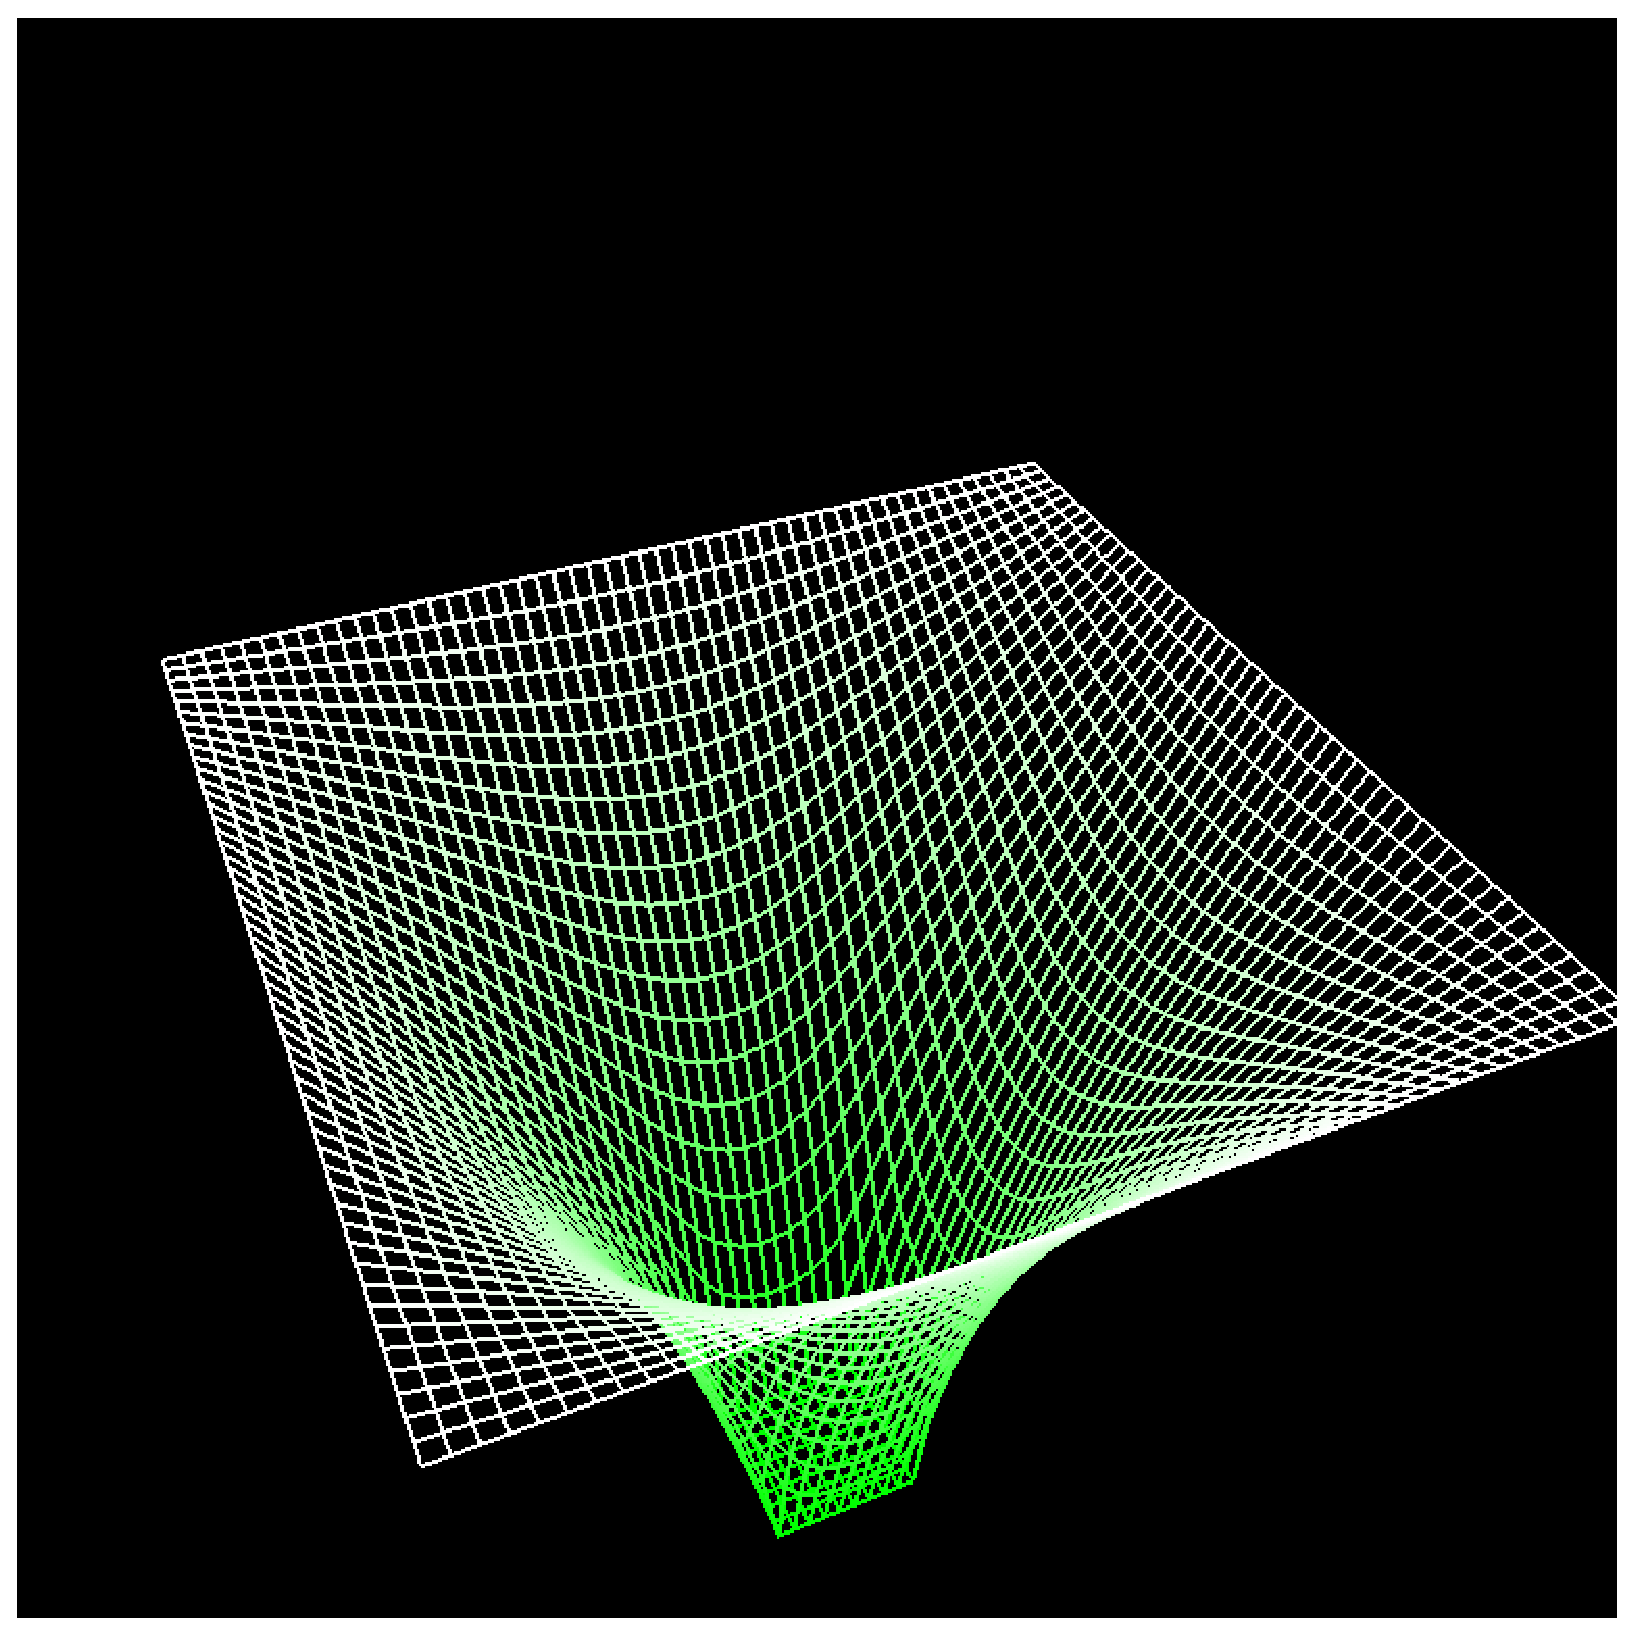
\includegraphics[scale=0.4]{im3}
\parbox{4in}{\emph{\caption{$n=50$, przewodnik w środku, ujemny potencjał przewodnika.}}}
\end{center}
\end{figure}
\end{document}
